% Maxime's TOC
%
% IR
% - HIR
% - IR types
% - LIR
% - IIR
%   - Annotations
%
% IR support: static definitions
% IR support: auto-generated code
% - layouts and their methods (alloc/init, accessors)
% - GC visit code
% - FFI wrappers
%
% Compilation phases
% - Present before IR?
% - Picture
%   - Parsing
%   - AST simplification/annotation
%   - AST->IR conversion
%   - IR lowering/optimization
%   - Register allocation
%   - Machine code generation
%
% Optimistic optimizations
% - Optimization issues
% - Getting rid of guards
% - Picture(s)
%   - Specialization
%   - Execution model
% - Less about type profiling?
% - Less about related work?

% TODO list:
% - [X] Wrap some lines, change undefined to undef, scale up listing text
% - [X] Cut type profiling slides
% - [X] Cut related work slides
% - [X] Add slide for C sum code. Question, in bold: Could we eliminate all
%       conditional checks from this program?

% -- Slide ---------------------------------------------------------------------
\begin{frame}
\frametitle{\bf High-Level IR}
    \begin{itemize}

        \item Core JS semantics expressed in terms of HIR instructions
        \begin{itemize}
            \item Act on boxed, high-level (dynamic) types
            \begin{itemize}
                \item Strings, numbers, objects, \ldots
            \end{itemize}
            \item May produce exceptions in some cases
        \end{itemize}

        \item Examples
        \begin{itemize}
            \item Arithmetic/comparison operators (\code{+}, \code{-},
            \code{==}, \ldots)
            \item Property accesses (getProp, putProp, hasProp, \ldots)
            \item Misc.~JavaScript operators (\code{typeof}, \code{instanceof}, \ldots)
        \end{itemize}

        \item Currently, HIR implemented directly by {\bf primitive functions}
        % \begin{itemize}
        %     \item Primitives written in terms of extended JS
        %     \item Annotated for performance
        %         \begin{itemize}
        %             \item Static linkage, force inlining, no exceptions, etc.
        %         \end{itemize}
        % \end{itemize}

    \end{itemize}
\end{frame}
% ------------------------------------------------------------------------------

\begin{frame}
\frametitle{\bf Primitive Functions}
    \begin{itemize}
        \item All Tachyon functions can use our extended JS, meaning:
        \begin{itemize}
            \item Special function annotations
            \item Typed local variables
            \item Inline IR (IIR) instructions
        \end{itemize}
        \item Core of the runtime makes more use of this
        \begin{itemize}
            \item Rest of Tachyon mostly uses `standard' JS
        \end{itemize}
        \item Annotations allow functions to:
        \begin{itemize}
            \item Have static linkage (no dynamic lookup)
            \item Always be inlined
            \item Be prevented from accessing the global object
            \item Use typed argument values
            \item Use a typed return value
        \end{itemize}
    \end{itemize}
\end{frame}

% -- Slide ---------------------------------------------------------------------
\begin{frame}
\lstinputlisting[language=JavaScript]{images/lt.js}
\end{frame}
% ------------------------------------------------------------------------------

% -- Slide ---------------------------------------------------------------------
\begin{frame}
\scalebox{1.2}{\lstinputlisting[language=JavaScript]{images/boxIsInt.js}}
\end{frame}
% ------------------------------------------------------------------------------

% -- Slide ---------------------------------------------------------------------
\begin{frame}[fragile]
\frametitle{\bf Tachyon's Extended JavaScript}
    \begin{itemize}
        \item JavaScript has no access to raw memory
        \begin{itemize}
            \item Essential to implement a VM/JIT
        \end{itemize}
        \item Tachyon is written in JS w/ “unsafe” extensions
        \begin{itemize}
            \item Minimizes the need to write C code (FFI)
            \item Exposes potential optimization opportunities
            \begin{itemize}
                \item FFIs are optimization boundaries
            \end{itemize}
        \end{itemize}
        \item JS code translated to low-level typed IR
        \begin{itemize}
            \item JS extension: insert inline IR (IIR) in source code
        \end{itemize}
    \end{itemize}

\begin{block}<+->{Inline IR example}
\begin{lstlisting}[language=JavaScript]
if (boxIsInt(v1) && boxIsInt(v2)) {
    // Compare immediate integers without unboxing
    var tv = iir.lt(v1, v2);
}
\end{lstlisting}
\end{block}
\end{frame}
% ------------------------------------------------------------------------------

% -- Slide ---------------------------------------------------------------------
\begin{frame}
\frametitle{\bf Low-Level IR}
    \begin{itemize}
        \item Some similarities with LLVM
        \item SSA-based
        \item Type-annotated
        \begin{itemize}
            \item Integers, floats, booleans, raw pointers
            \item Boxed values, references
        \end{itemize}
        \item Low-level
        \begin{itemize}
            \item Mirrors instructions commonly found on most CPUs
            \begin{itemize}
                \item add/sub/mul/div, and/or/shift, jump/if/call, load/store, etc.
            \end{itemize}
            \item Still tries to be “machine agnostic”
            \begin{itemize}
                \item No specific endianness, no registers
            \end{itemize}
            \item Allows expressing more optimizations (specialization)
        \end{itemize}
    \end{itemize}
\end{frame}
% ------------------------------------------------------------------------------

\begin{frame}
\frametitle{\bf IIR $\neq$ Assembly}
    \begin{itemize}
        \item Writing code using IIR not as painful as it sounds
        \item Using IIR does not take away JS capabilities!
        \begin{itemize}
            \item Still get dynamic typing, strings, closures
        \end{itemize}

        \item Don't need to annotate the type of every local variable

        \item Also facilitated by auto-generated code

        \item Auto-generated accessor methods for heap objects
        \begin{itemize}
            \item alloc\_str(len), get\_str\_len(str), get\_str\_data(str, i)
        \end{itemize}

        \item Auto-generated wrappers for C FFI wrappers
        \begin{itemize}
            \item puts('Hello World!'), malloc(size), free(ptr), exit(intval)
        \end{itemize}

    \end{itemize}
\end{frame}

\begin{frame}
\scalebox{0.9}{\lstinputlisting[]{images/newObject.js}} 
\end{frame}

\begin{frame}
\frametitle{\bf Foreign Function Interface (FFI)}
    \begin{itemize}
        \item Can both import and export functions

        \item Auto-generated wrapper functions
        \begin{itemize}
            \item Present C functions as JS functions
            \item Present JS functions as C functions
            \item Automatic type conversions
        \end{itemize}

        \item For now: C code never touches JS objects

        \item Minimal number of C functions exposed
        \begin{itemize}
            \item Memory management, file/console IO, profiling
        \end{itemize}

        \item Built for speed
        \begin{itemize}
            \item FFI calls are JITed and statically linked
            \item Wrapper functions are inlinable
        \end{itemize}

    \end{itemize}
\end{frame}

% -- Slide ---------------------------------------------------------------------
\begin{frame}
\frametitle{\bf V8 Extensions}

  \begin{itemize}

  \item Memory allocation (for data and code)
    \begin{itemize}
    \item {\tt allocMemoryBlock}, {\tt freeMemoryBlock}
    \item {\tt readFromMemoryBlock}, {\tt writeToMemoryBlock}
    \item {\tt execMachineCodeBlock}
    \end{itemize}

  \item I/O (for source code and REPL)
    \begin{itemize}
    \item {\tt readFile}, {\tt writeFile}
    \item {\tt readConsole}
    \end{itemize}

  \item Profiling
    \begin{itemize}
    \item {\tt currentTimeMillis}, {\tt memAllocatedKBs}
    \item {\tt pauseV8Profile}, {\tt resumeV8Profile}
    \item {\tt shellCommand}
    \end{itemize}

  \item FFI
    \begin{itemize}
    \item {\tt getFuncAddr} (to get {\tt puts}, {\tt malloc}, {\tt free}, {\tt
    runtimeError}, \ldots)
    \item {\tt getBlockAddr}
    \item {\tt callTachyonFFI}
    \end{itemize}

  \end{itemize}

\end{frame}
% ------------------------------------------------------------------------------

%
% Example of program JS->AST->HIR->LIR->ASM
%

\begin{frame}
\frametitle{\bf Example: Simple JS Function}
\lstinputlisting[language=JavaScript,basicstyle=\bfseries\Large\ttfamily]{images/ex_source.js}
\end{frame}

\begin{frame}[fragile]
\frametitle{\bf Example: Abstract Syntax Tree (AST)}
\scalebox{1.15}{\lstinputlisting[language=,keepspaces=true,basicstyle=\bfseries\tiny\ttfamily]{images/ex_ast.txt}}
\end{frame}

\begin{frame}
\frametitle{\bf Example: High-Level IR (HIR)}
\scalebox{0.8}{\lstinputlisting[language=,keepspaces=true,basicstyle=\bfseries\footnotesize\ttfamily]{images/ex_hir.txt}}
\end{frame}

\begin{frame}
\frametitle{\bf Example: Low-Level IR (LIR)}
\scalebox{0.8}{\lstinputlisting[language=,keepspaces=true,basicstyle=\bfseries\footnotesize\ttfamily]{images/ex_lir1.txt}}
\end{frame}

\begin{frame}
\frametitle{\bf Example: Low-Level IR (LIR) contd.}
\scalebox{0.8}{\lstinputlisting[language=,keepspaces=true,basicstyle=\bfseries\footnotesize\ttfamily]{images/ex_lir2.txt}}
\end{frame}

\begin{frame}
\frametitle{\bf Example: x86 Machine Code}
\begin{columns}[t]

\begin{column}{0.33\textwidth}
\scalebox{0.68}{\lstinputlisting[language=,keepspaces=true,basicstyle=\bfseries\footnotesize\ttfamily]{images/ex_asm1.txt}}
\end{column}

\begin{column}{0.33\textwidth}
\scalebox{0.68}{\lstinputlisting[language=,keepspaces=true,basicstyle=\bfseries\footnotesize\ttfamily]{images/ex_asm2.txt}}
\end{column}

\begin{column}{0.33\textwidth}
\scalebox{0.68}{\lstinputlisting[language=,keepspaces=true,basicstyle=\bfseries\footnotesize\ttfamily]{images/ex_asm3.txt}}
\end{column}

\end{columns}
\end{frame}

% -- Slide ---------------------------------------------------------------------
\begin{frame}
\frametitle{\bf Optimistic Optimizations}
    \begin{itemize}

        \item Traditional optimizations are conservative
        \begin{itemize}
            \item Can't prove it, can't do it
            \item Dynamic languages offer little static type information
            \item Dynamic constructs problematic for analysis
            \begin{itemize}
                \item \code{eval}, \code{load}
            \end{itemize}
            \item Often can't prove validity conservatively
        \end{itemize}

        \item Optimistic optimizations
        \begin{itemize}
            \item Most JavaScript programs not that dynamic
            \item Many optimizations do apply in practice
            \begin{itemize}
                \item But you can't always prove it conservatively
            \end{itemize}
            \item Valid now, presume valid until proven otherwise
            \begin{itemize}
                \item Innocent until proven guilty (faulty?)
            \end{itemize}

        \end{itemize}
    \end{itemize}
\end{frame}
% ------------------------------------------------------------------------------

% -- Slide ---------------------------------------------------------------------
\begin{frame}
\frametitle{\bf Example: Optimization Issues}
    \begin{center}
    \scalebox{1}{\lstinputlisting[language=JavaScript]{images/sum.js}}
    \end{center}
    \begin{itemize}
        \item Don't know type of \code{list} and its elements
        \item Type of \code{zero} could change
        \item Dynamic type checks needed
    \end{itemize}
\end{frame}
% ------------------------------------------------------------------------------

\begin{frame}
\frametitle{\bf Example: Dynamic Checks - Rough Sketch}
\scalebox{0.95}{\lstinputlisting[language=JavaScript]{images/sum_checks.js}}
\end{frame}

% -- Slide ---------------------------------------------------------------------
\begin{frame}
\frametitle{\bf What Would Tachyon Do (WWTD)?}
\begin{itemize}
    \item A VM can observe global variables types during execution
    \begin{itemize}
        \item Can assume that these types will not change
        \item Compile functions with these assumptions
    \end{itemize}

    \item A VM can observe function arguments types
    \begin{itemize}
        \item Can specialize functions based on these
    \end{itemize}

    \item Types inside of function bodies can be inferred from types of globals and arguments
    \begin{itemize}
        \item Type propagation, simple dataflow analysis
    \end{itemize}
\end{itemize}
\end{frame}
% ------------------------------------------------------------------------------

\begin{frame}
\frametitle{\bf Example: Guarded Code - Rough Sketch}
\scalebox{0.92}{\lstinputlisting[language=JavaScript]{images/sum_guarded.js}}
\end{frame}

% -- Slide ---------------------------------------------------------------------
%\begin{frame}
%\frametitle{\bf Realistic Assumptions}
%    \begin{itemize}
%        \item As programmers, it's fairly obvious to us that:
%        \begin{itemize}
%            \item function \code{f} is extremely unlikely to be redefined
%            \item \code{list} will likely always be array of integers
%        \end{itemize}
%
%        \item Not obvious to a compiler, but, in general:
%        \begin{itemize}
%            \item How often are global functions redefined?
%            \item How many call sites are truly polymorphic?
%            \item How many function arguments can have more than one type?
%            \item How often do people use eval to change local variable types?
%        \end{itemize}
%    \end{itemize}
%\end{frame}
% ------------------------------------------------------------------------------

% -- Slide ---------------------------------------------------------------------
\begin{frame}
\frametitle{\bf What Would Tachyon Do (WWTD)?}
\begin{center}
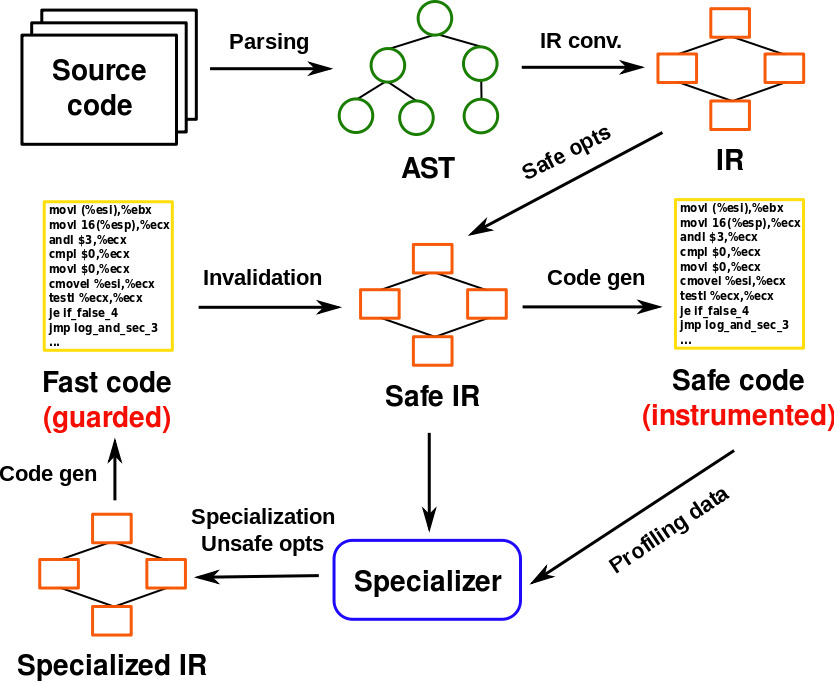
\includegraphics[width=3in]{images/transforms2}
\end{center}
\end{frame}
% ------------------------------------------------------------------------------

% -- Slide ---------------------------------------------------------------------
\begin{frame}
\frametitle{\bf Key Ideas}
    \begin{itemize}
        \item Crucial to capture info about run time behavior
        \begin{itemize}
            \item Tracing JITs do this, but leave many run time checks
        \end{itemize}

        \item Program needs to be correct at all times
        \begin{itemize}
            \item Don't need to run the same code at all times
            \item Multiple optimized versions correct at different times
        \end{itemize}

        \item Can make optimistic assumptions that may be invalidated
        \begin{itemize}
            \item So long as we can repair our mistakes in time
            \item Code with broken assumptions must never be executed
            \item Ideally, want invalidation to be unlikely
        \end{itemize}
    \end{itemize}
\end{frame}
% ------------------------------------------------------------------------------

% % -- Slide ---------------------------------------------------------------------
% \begin{frame}
% \frametitle{\bf Potential Difficulties}
%     \begin{itemize}
%         \item Cost of accurate type profiling
%         \begin{itemize}
%             \item Code-patching and self-limiting profiling
%         \end{itemize}
%         \item Cost of recompilation
%         \begin{itemize}
%             \item Usage of external threads
%         \end{itemize}
%         \item Frequency of recompilation
%         \begin{itemize}
%             \item Progressive pessimization
%         \end{itemize}
%         \item Inherent complexity
%         \begin{itemize}
%             \item Work hard!
%         \end{itemize}
%     \end{itemize}
% \end{frame}
% % ------------------------------------------------------------------------------

